\documentclass[a4paper, 12pt]{article}

\usepackage[T2A]{fontenc}
\usepackage[utf8]{inputenc}
\usepackage[english, russian]{babel}
\usepackage{amsmath}
\usepackage{graphicx}
\usepackage{subcaption}
\usepackage{float}
\usepackage{tabularx}
\usepackage{amsmath,booktabs}
\usepackage{array}
\righthyphenmin=2
\usepackage[left=20mm, top=20mm, right=20mm, bottom=20mm]{geometry} % настройки полей документа
\usepackage{caption}
\usepackage{makecell}

% Paragraph indent
\usepackage{indentfirst}
\setlength{\parindent}{15mm}

%%%%%%%TITUL%%%%%%%
\newcommand\tline[2]{$\underset{\text{#1}}{\text{\underline{\hspace{#2}}}}$}

%%%%%%%%%%%%CAPTION%%%%%%%
\usepackage{threeparttable}
%Change label separator
\usepackage{caption}
\captionsetup[table]{labelformat=simple, labelsep = endash, justification = raggedright, singlelinecheck = off, width = 0.75\textwidth}
\captionsetup[figure]{labelformat=simple, labelsep = endash, name = Рисунок}
%%%%%%%TABLE%%%%
\renewcommand{\arraystretch}{1.3}
\renewcommand{\tabcolsep}{0.7cm}

%%%%%%%%%%%%%%%%%%%%%%%%%%%%%%%%%%
\begin{document} 
	
		\begin{titlepage}
		\centering
		{\fontsize{12pt}{5cm}\selectfont \bfseries Министерство образования и науки Российской Федерации} \\ \vspace{0.5cm}
		{\fontsize{7pt}{5cm}\selectfont ФЕДЕРАЛЬНОЕ ГОСУДАРСТВЕННОЕ АВТОНОМНОЕ ОБРАЗОВАТЕЛЬНОЕ УЧРЕЖДЕНИЕ ВЫСШЕГО ПРОФЕССИОНАЛЬНОГО ОБРАЗОВАНИЯ} \\ 
		\vspace{1cm}
		{\fontsize{12pt}{5cm}\selectfont \bfseries САНКТ-ПЕТЕРБУРГСКИЙ УНИВЕРСИТЕТ ИНФОРМАЦИОННЫХ ТЕХНОЛОГИЙ, МЕХАНИКИ И ОПТИКИ} \\ \vspace{1.5cm}
		
		{\fontsize{14pt}{5cm}\selectfont Кафедра \hspace{1cm} \underline{Систем Управления и Информатики}  \hspace{1cm} Группа \underline{Р3340}} \\ 
		\vspace{2cm}
		
		{\fontsize{20pt}{5cm}\selectfont \bfseries Лабораторная работа №11} \\
		{\fontsize{20pt}{5cm}\selectfont \bfseries “Исследование математической модели пьезоэлектрического исполнительного устройства”} \\
		{\fontsize{14pt}{5cm}\selectfont Вариант - 02} \\
		\vspace{1.5cm}
		
		\flushleft
		
		{Выполнил \hspace{0.5cm} \tline{(фамилия, и.о.)}{10cm} (подпись)} \\
		\vspace{2cm}
		
		{Проверил \hspace{0.5cm} \tline{(фамилия, и.о.)}{10cm} (подпись)} \\
		\vspace{5cm}
		
		"\underline{\hspace{0.4cm}}"\hspace{0.1cm}\underline{\hspace{1.5cm}}\hspace{0.1cm}20\underline{\hspace{0.4cm}}г. \hspace{2cm} Санкт-Петербург, \hspace{2cm} 20\underline{\hspace{0.4cm}}г. \\ \vspace{1cm}
		
		Работа выполнена с оценкой \hspace{0.5cm} \underline{\hspace{10cm}} \\ 
		\vspace{1cm}
		Дата защиты "\underline{\hspace{0.4cm}}"\hspace{0.1cm}\underline{\hspace{1.5cm}}\hspace{0.1cm}20\underline{\hspace{0.4cm}}г.
		
		\end{titlepage}

\section*{Цель работы}
Целью работы является изучение математических моделей и исследование характеристик исполнительного устройства, построенного на основе пьезоэлектрического двигателя микроперемещений.

\section*{Исходные данные}
На рисунке \ref{first} приведена структурная схема пьезоэлектрического двигателя, параметры двигателя - таблица \ref{tab:dateTab}

\begin{table}[h!]
	\centering
	\begin{threeparttable}
		\caption{Исходные данные}
		\begin{tabular}{|c|c|c|c|c|c|}
			\hline
			\makecell{$C_p,$\\Н/м} & \makecell{$m,$\\кг} & \makecell{$K_0,$\\Н/В} & \makecell{$K_d,$\\Н$\cdot$с/м} & \makecell{$T_u,$\\мс} & \makecell{$F_B,$\\Н}\\
			\hline
			$0,5\cdot10^8$ & 0,3 & 8,2 & $0,9\cdot10^3$ & $0,06$ & 80\\
			\hline	
		\end{tabular}
		\label{tab:dateTab}
	\end{threeparttable}
\end{table}

\begin{figure}[h!]
	\centering
	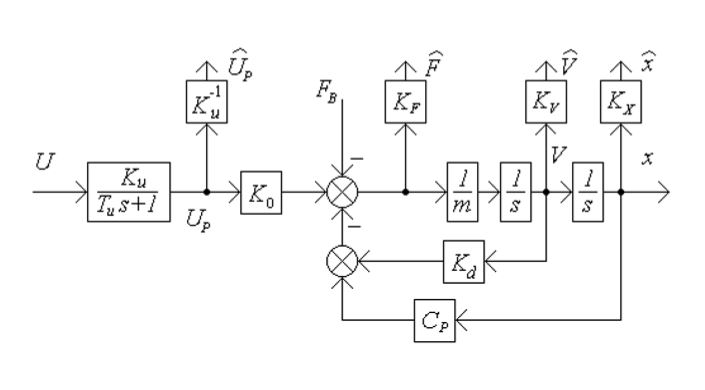
\includegraphics[width = 0.65\textheight]{first}
	\caption{Структурная схема пьезоэлектрического исполнительного устройства}
	\label{first}
\end{figure}

Коэффициенты передачи измерительных устройств $K_u^{-1}, K_F, K_V \text{и} K_x$ выбираются таким образом, чтобы обеспечить соответствие максимального значения измеряемого сигнала уровню 10 В на выходе измерительного устройства. В итоге получим следующие значения коэффициентов:

\begin{gather}
	K_u = 30\\
	K_F = 0.0081\\
	K_V = 22.9382\\
	K_x = 2.03267*10^5	
\end{gather}

\newpage


\begin{center}
	\section{Исследование исполнительного устройства}
\end{center}

Составим математическую модель в относительно исходных данных и получившихся значений коэффициентов. Модель представлена на рисунке \ref{funkshem}, а на рисунке \ref{begin} - графики переходных процессов при нулевом внешнем воздействии. 

\begin{figure}[h!]
	\centering
	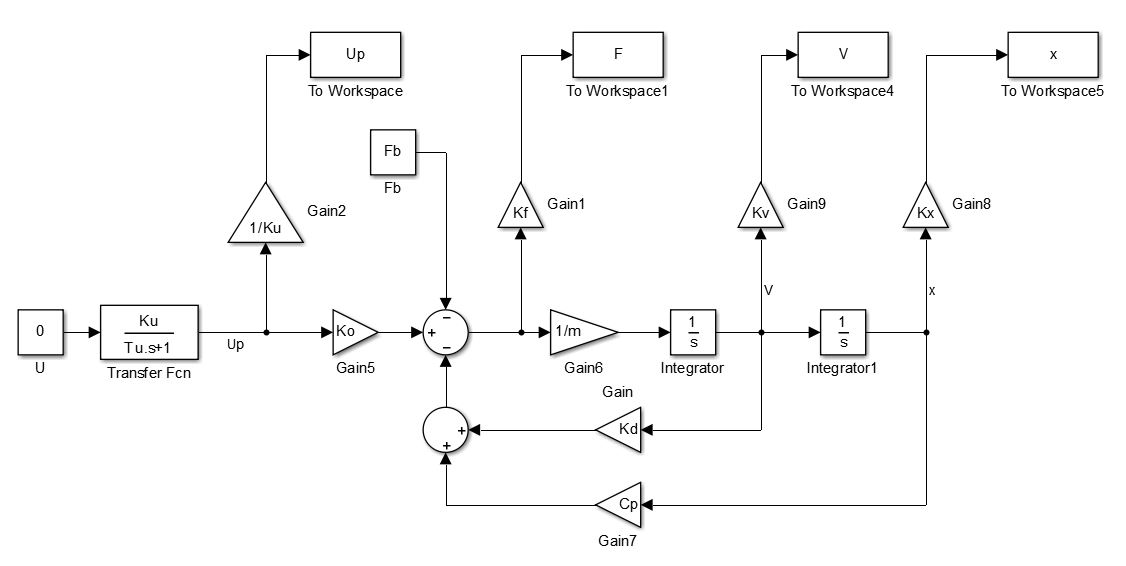
\includegraphics[width = 0.6\textheight]{funkshem}
	\caption{Функциональная схема пьезоэлектрического исполнительного устройства}
	\label{funkshem}
\end{figure}

\begin{figure}[h!]
	\centering
	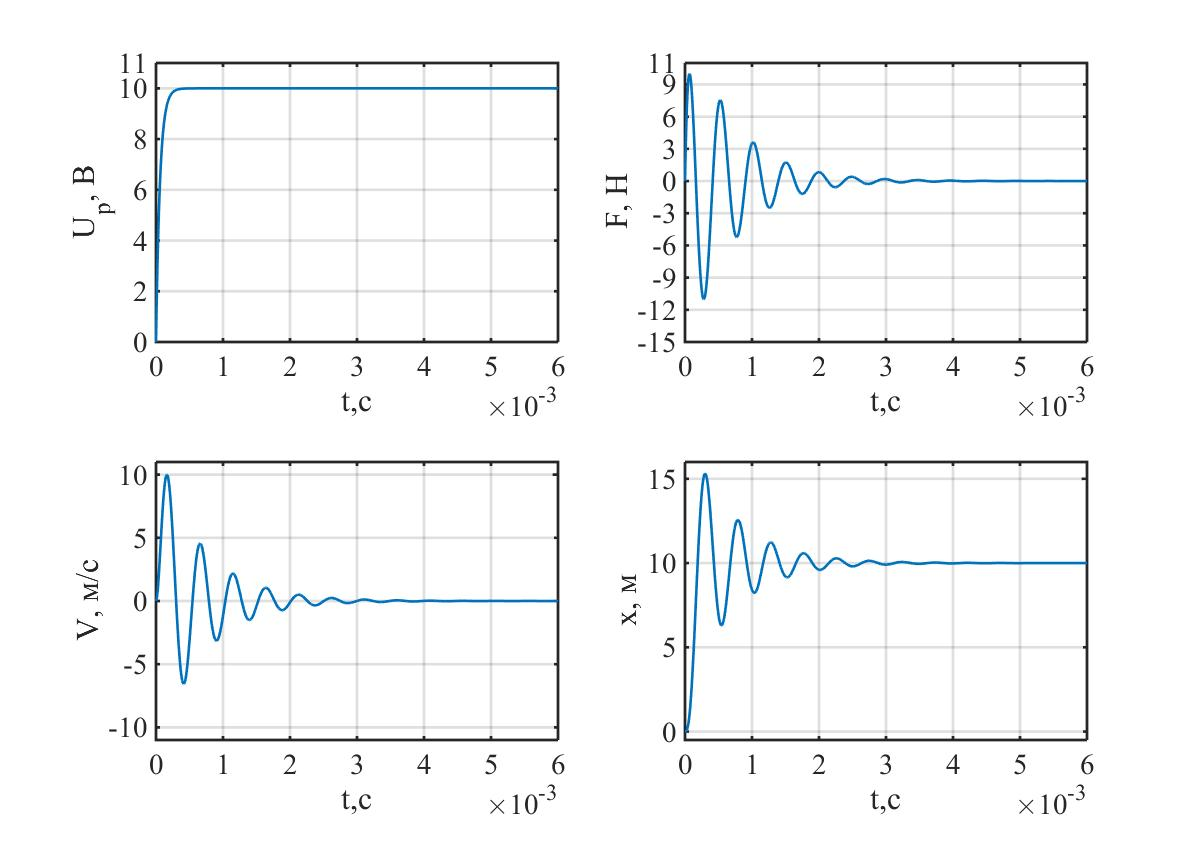
\includegraphics[width = 0.65\textheight]{data/begin}
	\caption{Переходные процессы при $F_b=0$ H $U=10$ B}
	\label{begin}
\end{figure}

\newpage

\begin{center}
	\section{Исследование влияния массы нагрузки на вид переходных процессов}
\end{center}\par

На рисунке \ref{m_x} показаны переходные процессы при различных значениях массы нагрузки. В таблице \ref{tab:x_m} приведена зависимость  характеристик системы от массы нагрузки.

\begin{figure}[h!]
	\centering
	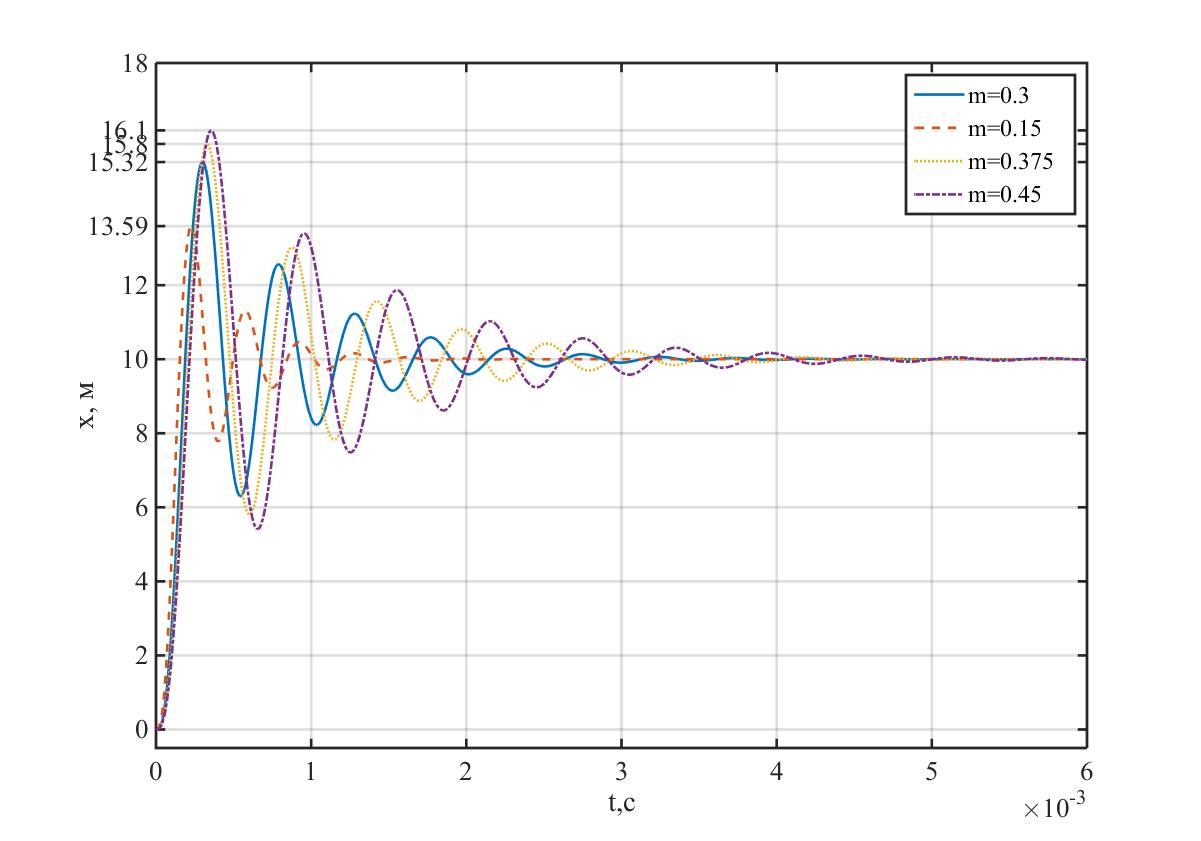
\includegraphics[width = 0.65\textheight]{data/m_x}
	\caption{Переходные процессы при изменении массы}
	\label{m_x}
\end{figure}

\begin{table}[ht!]
	\centering
	\begin{threeparttable}
		\caption{Данные переходных процессов при изменяющейся массе нагрузки}
		\begin{tabular}{|c|c|c|c|}
			\hline
			$m,$ кг	& $t_\text{п}, c$	& $\sigma, \%$	& $x_\text{у}$\\\hline
			0,15	& 0,8				& 35,9			& 10\\
			\hline
			0,3		& 1,81				& 53,2			& 10\\
			\hline
			0,375	& 2,29				& 58,1			& 10\\
			\hline
			0,45	& 2,79				& 61,9			& 10\\
			\hline
		\end{tabular}
		\label{tab:x_m}
	\end{threeparttable}
\end{table}

\newpage

\begin{center}
	\section{Исследование влияния постоянной времени на вид переходных процессов}
\end{center}\par

Передаточная функция системы:\\
\begin{equation}
	W(s)=\frac{K_UK_0}{T_Ums^3+(m+K_dT_U)s^2+(K_d+C_pT_U)s+C_p}
	\label{func}
\end{equation}\par

В таблице  приведена зависимость характеристик системы от постоянной времени и расчитанные корни передаточной функции \ref{func}.  

\begin{table}[ht!]
	\centering
	\begin{threeparttable}
		\caption{Данные переходных процессов при изменяющейся постоянной времени}
		\renewcommand{\arraystretch}{1.3}
		\renewcommand{\tabcolsep}{0.45cm}
		\begin{tabular}{|c|c|c|c|c|c|c|}
			\hline
			$T_u,$ мс	& $t_\text{п},$ мс	& $\sigma, \%$	& $x_y$	& $s_1$		& $s_2$								& $s_3$								\\
			\hline
			0,06		& 1,8				& 53,2			& 10	& -16666,67	&-1500 + j12822,5	& -1500 - j12822,5\\
			\hline
			0,12		& 1,6				& 30,1			& 10	& -8333,33	&-1500 + j12822,5	& -1500 - j12822,5\\
			\hline
			0,24		& 1,2				& 6,1			& 10	& -4166,67	&-1500 + j12822,5	& -1500 - j12822,5\\
			\hline
			0,36		& 1,1				& 0,7			& 10	& -2777,78	&-1500 + j12822,5	& -1500 - j12822,5\\
			\hline
		\end{tabular}
		\label{tvarTab}
	\end{threeparttable}
\end{table}\par

На рисунке \ref{Tu_x} показаны переходные процессы при различных значениях массы нагрузки.

\begin{figure}[h!]
	\centering
	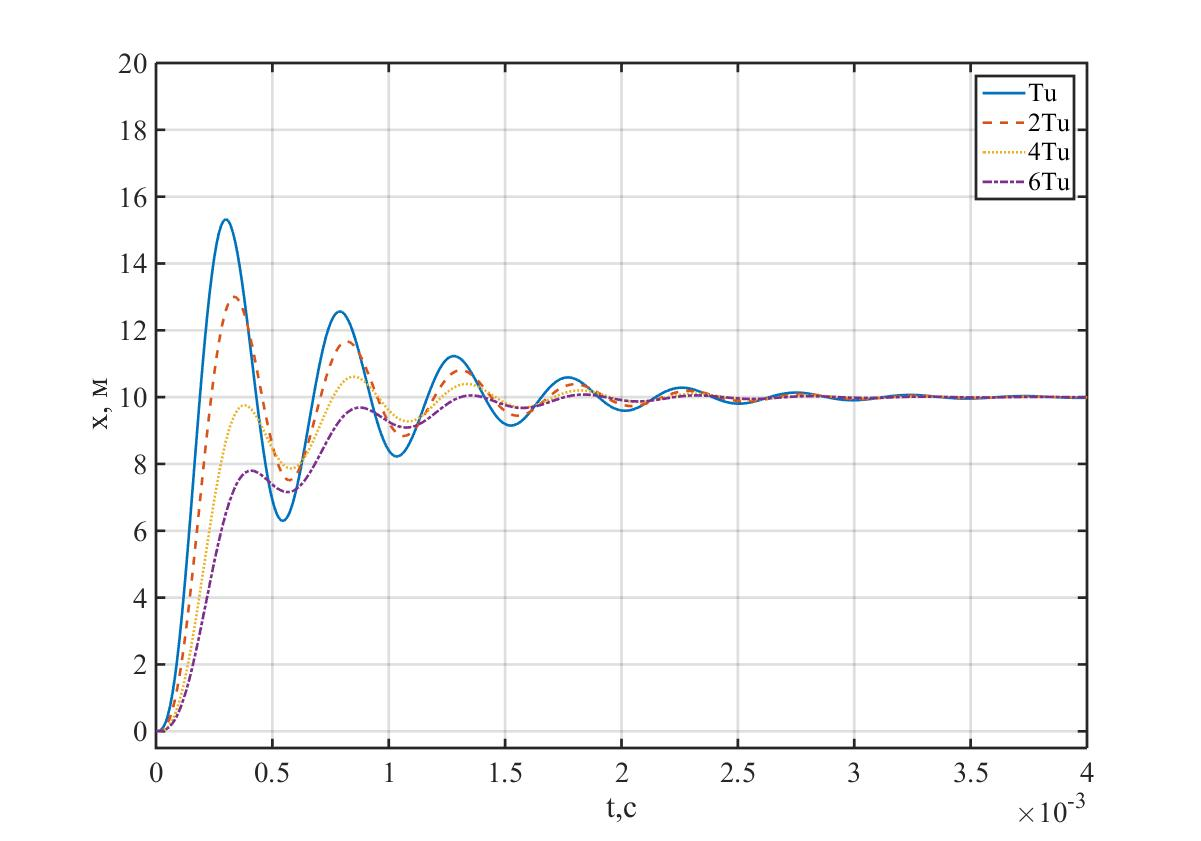
\includegraphics[width = 0.65\textheight]{data/Tu_x}
	\caption{Переходные процессы при изменении постоянной времени}
	\label{Tu_x}
\end{figure}

\newpage

\begin{center}
	\section{Исследование влияния коэффициентов упругости на вид переходных процессов}
\end{center}\par

На рисунках \ref{Cp_V} и \ref{Cp_x} показаны переходные процессы по скорости и положению, относительно коэффициента упругости.

\begin{figure}[h!]
	\centering
	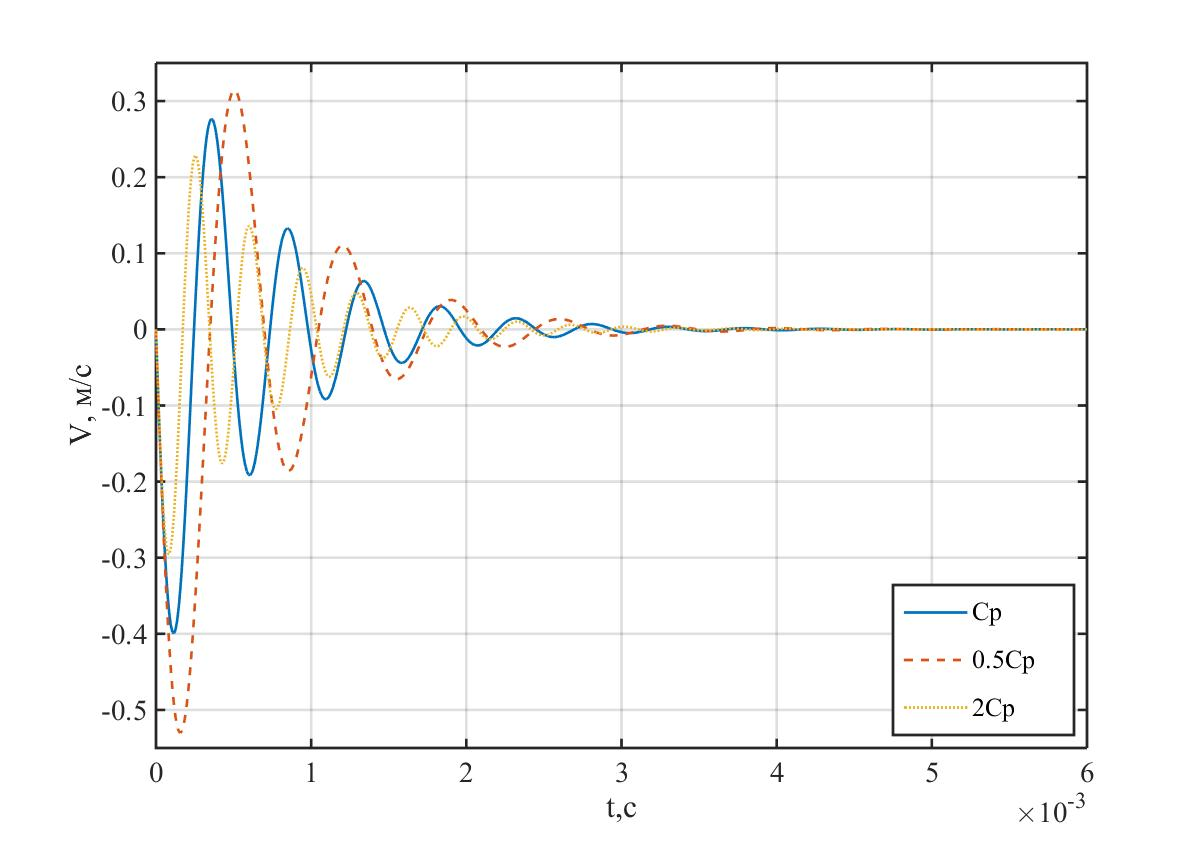
\includegraphics[width = 0.65\textheight]{data/Cp_V}
	\caption{Переходные процессы при изменении коэффициента упругости}
	\label{Cp_V}
\end{figure}

\newpage

\begin{figure}[h!]
	\centering
	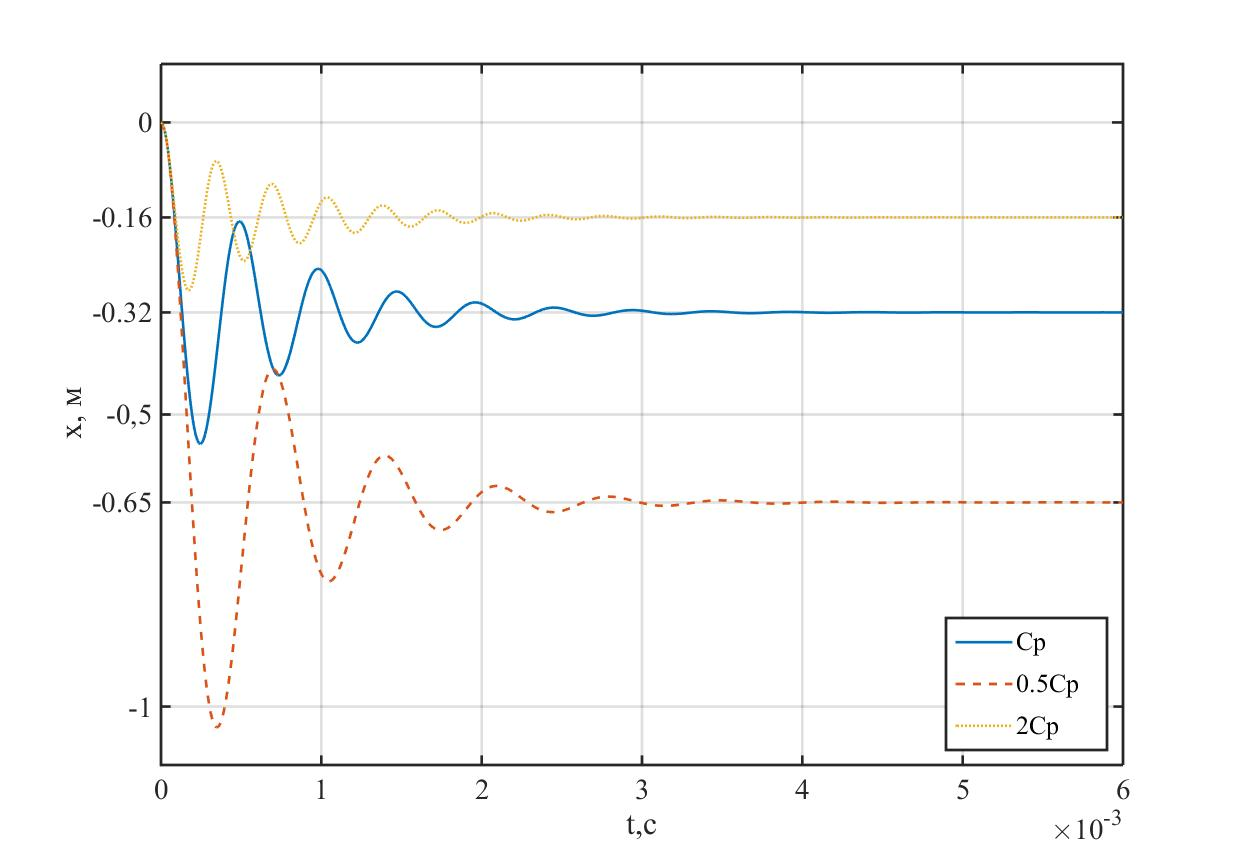
\includegraphics[width = 0.65\textheight]{data/Cp_x}
	\caption{Переходные процессы при изменении коэффициента упругости}
	\label{Cp_x}
\end{figure}

\newpage

\begin{center}
	\section{Построение ЛАЧХ исполнительного устройства}
\end{center}\par

Представим асипмтотическую логарифмическую характеристику для нашей системы в виже колебательного звена:

\begin{align}
	W(s) = \frac{\displaystyle{\frac{K_0}{C_p}}}{\displaystyle{\frac{m}{C_p}}s^2 + \frac{K_d}{C_p}s + 1}.
\end{align}

На рисунке \ref{lachx} видно где асимптотическая ЛАЧХ имеет нулевой наклон и после какой частоты ее наклон составляет -40 дБ/дек.

\begin{figure}[h!]
	\centering
	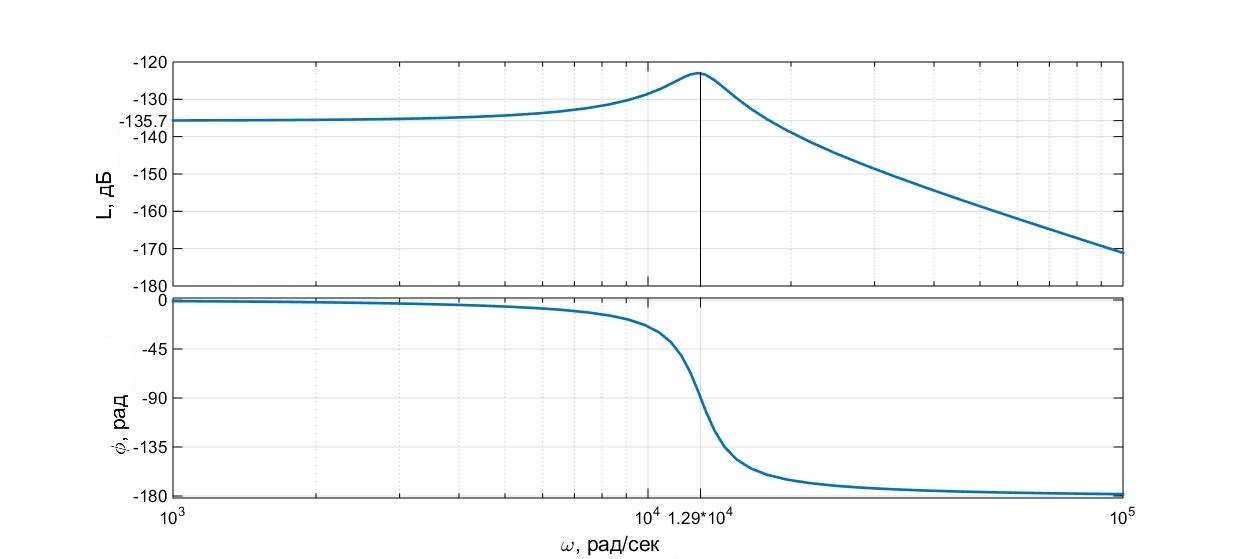
\includegraphics[width = 0.65\textheight]{data/lachx}
	\caption{Асимптотическая ЛАЧХ}
	\label{lachx}
\end{figure}

\newpage

\begin{center}
	\section*{Вывод}
\end{center}\par
В лабораторной работе было исследовано пьезоэлектрическое устройство, которое можно представить в виде колебательного звена.\par
При исследовании влияния массы нагрузки на пьезоэлектрическое устройство, было выявлено, что при ее увеличении, увеличивается время переходного процесса\par
При изменении постоянной времени изменяется время переходного процесса и перерегулирование. При увеличении $T_u$, растет $t_\text{п}$ и убывает $\sigma$, установившееся значение остается неизменным.\par
При исследовании коэффициента упругости было выявлено, что, при увеличении $C_p$, увеличивается колебательность системы без изменения времени переходного процесса.



\end{document} 